\newpage 

\section{Memory Hierarchy Optimizations}

Software-controlled data prefetching is a promising technique for
improving the performance of the memory subsystem to match
today’s high-performance processors. While prefctching is useful in
hiding the latency, issuing prefetches incurs an instruction overhead
and can increase the load on the memory subsystem. As a resu 1~
care must be taken to ensure that such overheads do not exceed the
benefits.


\subsection{Introduction}

Various hardware and software approaches to improve the memory
performance have been proposed recently [15]. A promising technique 
to mitigate the impact of long cache miss penalties is softwarecontrolled
 prefetching[5, 13, 16, 22 23]. Software-controlled
prefetching\cite{mowry1992design} requires support from both hardware and software. The
processor must provide a special “prefetch” instruction. The software 
uses this instruction to inform the hardware of its intent
to use a particular data item, if the data is not cumently in the
cache, the data is fetched in from memory. The cache must be
lockup-free[17]; that is, the cache must allow multiple outstrmding
 misses. While the memory services the data miss, the program
can continue to execute as long as it does not need the requested
data. While prefetching does not reduce the latency of the memory
access, it hides the memory latency by overlapping the access with
computation and other accesses. Prefetches on a scalar machine
are analogous to vector memory accesses on a vector machine. In
both cases, memory accesses are overlapped with computation and
other accesses. Furthermore, similar to vector registers, prefetching
allows caches in scalar machines to be managed by software. A
major difference is that while vedor machines can only operate on
vectors in a pipelined manner, scalar machines can execute arbitrary
sets of scalar operations well.


Another useful memory hierarchy optimization is to improve data
locality by reordering the execution of iterations. One important
example of such a transform is blocking[l, 9, 10, lZ 21, 23, 29].
Instead of operating on entire rows or columns of an array, blocked
algorithms operate on submatrices or blocks, so that datu loaded
into the faster levels of the memory hkmarchy are reused. Other
useful transformations include unimodular loop transforms such as
interchange, skewing and reversal[29]. Since these optimization
improve the @de’s data locality, they not only reduee the effeetive
 memory access time but also reduce the memory bandwidth
requirement. Memory hierarchy optimization such as prefetching
and blocking are crucial to turn high-performance microprocessors
into effective scientific engines.



\subsection{Blocking\cite{lam1991cache}}


Blocking is a well-known optimization technique for improving
the effectiveness of memory hierarchies. Instead of operating on
entire rows or columns of an array, blocked algorithms operate on
submatrices or blocks, so that data loaded into the faster levels
of the memory hierarchy are reused. This paper presents cache
performance data for blocked programs and evaluates several optimization 
to improve this performance. The data is obtained by
a theoretical model of data conflicts in the cache, which has been
validated by large amounts of simulation.

Due to high level integration and superscalar architectural designs,
the floating-point arithmetic capability of microprocessors has increased significantly in the last few years. Unfortunately, the increase in processor speed has not been accompanied by a similar
increase in memory speed. To fully realize the potential of the
processors, the memory hierarchy must be efficiently utilized.

While data caches have been demonstrated to be effective for
general-purpose applications in bridging the processor and memory speeds, their effectiveness for numerical code has not been
established. A distinct chmactenstic of numerical applications is
that they tend to operate on large data sets. A cache may only be
able to hold a small fraction of a matrix; thus even if the data are
reused, they may have been displaced from the cache by the time
they are reused.

Consider the example of matrix multiplication for matrices of size
NxN:

\begin{figure}[H]
	\centering
	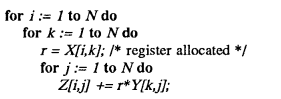
\includegraphics[width=0.6\textwidth]{p194.png}
	\caption{matrix multiplication example}
	\label{fig:p194}
\end{figure}



Figure \ref{fig:p193}(a) shows the data access pattern of this code. The same
element $X[i,k]$ is used by all iterations of the innermost loop; it
can be register allocated and is fetched from memory only once.
Assuming that the matrix is organized in row major order, the
innermost loop of this code accesses consecutive data in the Y
and $Z$ matrices, and thus utilizes the cache prefetch mechanism
fully. The same row of $Z$ accessed in an innermost loop is reused
in the next iteration of the middle loop, and the same row of
$Y$ is reused in the otftermost loop. Whether the data remains in
the cache at the time of reuse depends on the size of the cache.
Unless the cache is large enough to hold at least one $N * N$
matrix, the data Y would have been displaced before reuse. If
the cache cannot hold even one row of the data then $Z$ data in
the cache cannot be reused. In the worst case, $2N^3 + N^2$ words
of data need to be read from memory in $N^3$ iterations. The high
ratio of memory fetches to numerical operations can significantly
slow down the machine.


\begin{figure}[H]
	\centering
	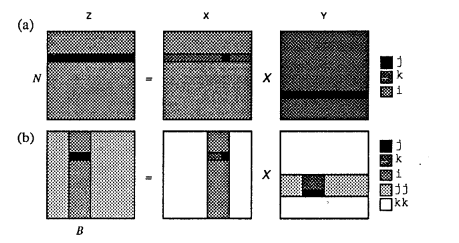
\includegraphics[width=0.6\textwidth]{p193.png}
	\caption{Data access pattern in (a) unblocked and (b) blocked matrix multiplication.}
	\label{fig:p193}
\end{figure}


It is well known that the memory hierarchy can be better 
utilized if scientific algorithms are blocked.
Blocking is also known as tiling. 
Instead of operating on individual matrix entries, 
the calculation is performed on submatrices.


Blocking can be applied to any and multiple levels of memory
hierarchy, including virtual memory, caches, vector registers, and
scalar registers. The matrix multiplication code
blocked to reduce cache misses looks like this:

\begin{figure}[H]
	\centering
	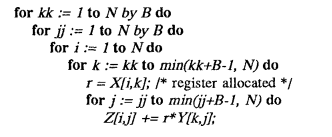
\includegraphics[width=0.6\textwidth]{p195.png}
	\caption{Reduced matrix multiplication example.}
	\label{fig:p195}
\end{figure}


Figure \ref{fig:p193}(b) shows the data access pattern of the 
blocked code. We
observe that the original data access pattern is reproduced here,
but at a smaller scale. The blocking factor, $B$ , is chosen so that
the $B * B$ submatrix of $Y$ and a row of length $B$ of $Z$ can fit in
the cache. In this way, both $Y$ and $Z$ are reused $B$ times each time
the data rue brought in. Thus, the total memory words accessed
is $2N^3/B + N2$ if there is no interference in the cache.

Blocking is a general optimization technique for increasing the
effectiveness of a memory hierarchy. By reusing data in the faster
level of the hierarchy, it cuts down the average access latency.
It also reduces the number of references made to slower levels
of the hierarchy. Blocking is thus superior to optimization such
us prefetching, which hides the latency but does not reduce the
memory bandwidth requirement. This reduction is especially important for multiprocessors since memory bandwidth is often the
bottleneck of the system.

\subsection{Prefetch\cite{mowry1992design}}
In this section, we will use the code in Figure \ref{fig:p196}(a) as a running
example to illustrate our prefetch algorithm. We assume, for this
example, that the cache is 8K bytes, the prefetch latency is 100
cycles and the cache line size is 4 words (two double-word array 
elements to each cache line), In this case, the set of references 
that will
cause cache misses can be determined by inspection (Figure \ref{fig:p196}(b)).

\begin{figure}[H]
	\centering
	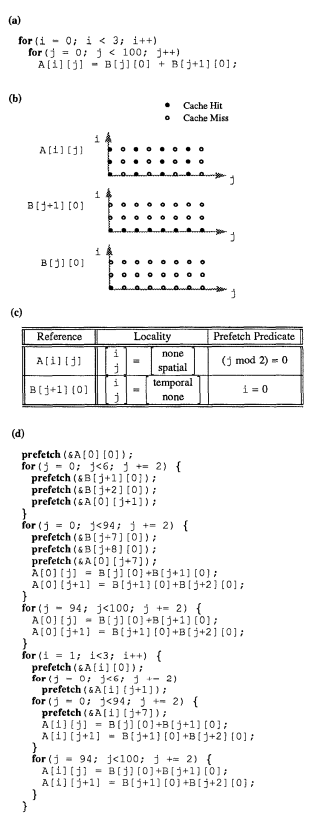
\includegraphics[width=0.6\textwidth]{p196.png}
	\caption{Example of selective prefetching algorithm.}
	\label{fig:p196}
\end{figure}

In Figure \ref{fig:p196}(d), we show code that issues all the useful prefetches
early enough to overlap the memory accesses with computation on
other data. (This is a source-level representation of the actual co
generated by our compiler for this case). 
The first three loops correspond to the computation 
of the i=O iteration, and the remaining
code executes the remaining iterations. 
This loop splitting step is
necessary because the prefetch pattern is different 
for the different
iterations. Furthermore, 
it takes three loops to implement the innermost loop. The first 
loop is the prolog, which prefetches data for
the initial set of iterations; the second loop is the steady state where
each iteration executes the code for the iteration and prefetches for
future iterations; the third loop is the epilog that executes the last
iterations. This so~are pipelining transformation is necessary to
issue the prefetches enough iterations shead of their use[18, 24].

This example illustrates the three major steps in the prefetch
algorithm
\begin{itemize}


\item 1. For each reference, determine the accessesthat are likely to be
cache misses and therefore need to be prefetched.
\item 2. Isolate the predicted cache miss instances through loop splitting. This avoids the overhead of adding conditional statements
to the loop bodies.
\item 3. Software pipeliie prefetches for all cache misses.

\end{itemize}

In the following, we describe each step of the algorithm and show
how the algorithm develops the prefetch code for the above example
systematically.

\subsubsection{Locality Analysis}

The tirst step determines those references that are likely to cause a
cache miss, This locality analysis is broken down into two substeps.
The tirst is to discover the intrinsic data reuses within a loop nest;
the second is to determine the set of reuses that cart be exploited
by a cache of a particular size.


\paragraph{Reuse Analysis}


Reuse analysis attempts to discover those instances of array accesses
that refer to the same cache line. There are three kinds of reuse:
temporal, spatial and group. In the above example, we say that
the reference A [i][j] has spatial reuse within the innermost loop
since the same cache line is used by two consecutive iterations in
the innermost loop. The reference B [j][0] has temporal reuse in
the outer loop since iterations of the outer loop refer to the same
locations. Lastly, we say that different accesses B [j][0] and
B [j+ 1][0] have group reuse because many of the instances of
the former refer to locations accessed by the latter.

Trying to determine accurately all the iterations that use the same
data is too expensive. We can succinctly capture our intuitive 
characterization that reuse is carried by a specific loop with the following mathematical formulation. We represent an n-dimensional loop
nest as a polytope in an n-dimensional iteration space, with the
outermost loop represented by the first dimension in the space. We
represent the’ shape of the set of iterations that use the same data
by a reuse vector space[291.


For example, the access of b[j][0] in our example is represented 
as \( B\left(\left[\begin{array}{ll}
	0 & 1 \\
	0 & 0
	\end{array}\right]\left[\begin{array}{l}
	i \\
	j
 	\end{array}\right]\right) \), 
so reuse occurs between iterations \((i_1,j_1)\) and \((i_2,j_2)\) 
whenever

$$
\begin{gathered}
{\left[\begin{array}{ll}
0 & 1 \\
0 & 0
\end{array}\right]\left[\begin{array}{l}
i_1 \\
j_1
\end{array}\right]=\left[\begin{array}{ll}
0 & 1 \\
0 & 0
\end{array}\right]\left[\begin{array}{l}
i_2 \\
j_2
\end{array}\right], \text { or }} \\
{\left[\begin{array}{ll}
0 & 1 \\
0 & 0
\end{array}\right]\left[\begin{array}{c}
i_1-i_2 \\
j_1-j_2
\end{array}\right]=\left[\begin{array}{l}
0 \\
0
\end{array}\right] .}
\end{gathered}
$$


That is, temporal reuse occurs whenever the difference between
the two iterations lies in the nullspace of \(
	\left[\begin{array}{ll}
		0 & 1 \\
		0 & 0
		\end{array}\right] \), that is,
span ${(1, O)}$. We refer to this vector space as the temporal reuse
vector space. This mathematical approach succinctly captures the
intuitive concept that the direction of reuse of B [j][0] lies along
the outer loop. This approach can handle more complicated access
patterns such as C[i+j] by representing their reuse vector space
as Span${ (1, -1)}$.

Similar analysis can be used to find spatial reuse. For reuse
among different array references, Gannon et al. observe that data
reuse is exploitable only if the references are uniformly generated,
that is, references whose array index expressions differ in at most
the constant term[11]. For examplq references B [j][0] and
B[j+1][0] are uniformly generatd, references C [i] and C [j]
are not. Pairs of uniformly generated references can be analyzed in
a similar fashion[29]. For our example in Figure \ref{fig:p196}(a), our algorithm
will determine that A [i] [j] has spatird reuse on the inner loop,
and both B[j] [0] and B[j+l] [0] share group reuse wtd also
have temporal reuse on the outer loop.

\paragraph{Localized Iteration Space}


Reuses translate to locality only if the subsequent use of data occurs
before the data are displaced from the cache. Factors that determine
if reuse translates to locality include the loop iteration count (since
that determines how much data are brought in between reuses), the
cache size, its set associativity and replacement policy.

We begin by considering the first two factors: the loop iteration
count and the cache size. In the example above, reuse of B [j][0]
lies along the outer dimension. If the iteration count of the innermost loop is large relative to the cache size (e.g., if the upper bound
of the $j$ loop in Figure \ref{fig:p196}(a) was 10,000 rather than 100), the data
may be flushed from the cache before they are used in the next outer
iteration. It is impossible to determine accurately whether data will
remain in the cache due to factors such as symbolic loop iteration
counts and the other cache characteristics. Instead of trying to represent exactly which reuses would result in a cache hi~ we capture
only the dimensionality of the iteration space that has data locality [’291.We define the localized iteration space to be the set of
loops that can exploit reuse. For example, if the localized iteration
space consists of only the innermost loop, that means data fetched
will be available to iterations within the same innermost loop, but
not to iterations from the outer loops.

The localized iteration space is simply the set of innermost loops
whose volume of data accessed in a single iteration does not exceed
the cache size. We estimate the amount of data used for each level
of loop nesting, using the reuse vector information. Our algorithm
is a simplified version of those proposed previously[8, 11, 23]. We
assume loop iteration counts that cannot be determined at compile
time to be small-this tends to minimize the number of prefetches. A reuse can be exploited
only if it lies within the localized iteration space. By representing
the localized iteration space also as a vector space, locality exists
only if the reuse vector space is a subspace of the localized vector
space

Consider our example in Figure \ref{fig:p196}(a). In this case, the loop bound
is known so our algorithm can easily determine that the volume of
data used in each loop fits in the cache. Both loops are within
the localized iteration space, and the localized vector space is represented as span 
${( 1, 0), (0, 1)}$. Since the reuse vector space is necessarily 
a subspace of the localizad vector space, the reuses will
correspond to cache hits, and it is not necessary to prefetch the
reuses.

Similar mathematical treatment determines whether spatial reuse
translates into spatial locality. For group reuses, our algorithm
determines the sets among the group that can exploit locality using
a similar technique. Furthermore, it determines for each set its
leading reference, the reference that accesses new data first and is
thus likely to incur cache misses. For example, of B [j ] [ 0] and
B [ j+1 ] [ 0],B [ j+1 ] [ 0] is the first reference that accesses new
data. The algorithm need only issue prefetches for B [ j+1 ] [ 0]
and not B [j ] [ 0].


In the dkcussion so far, we have ignored the effects of cache
conflicts. For scientific programs, one important source of cache
conflicts is due to accessing data in the same matrix with a constant
stride. Such conflicts can be predicted, and can even be avoided by
embedding the matrix in a larger matrix with dimensions that are
less problemztic[19]. We have not implemented this optimization in
our compiler. Since such interference can greatly disturb our simulation results, we manually changed the size of some of the matrices
in the benchmarks (details are given in Section 3.) Conflicts due
to interference between two different matrices are more difficult to
analyze. We cumently approximate this effect simply by setting the
“effective” cache size to be a fraction of the actual cache size.


\paragraph{The Prefetch Predicate}

The benefit of locality differs according to the type of reuse. If an
access has temporal locality within a loop nest, only the first access
will possibly incur a cache miss. If an access has spatial locality,
only the ftrst access to the same cache line will incur a miss.

To simplify this exposition, we assume here that the iteration
count starts at 0, and that the data arrays are aligned to start on
a cache line boundary. Without any locality, the default is to
prefetch all the time. However, the presence of temporal locality 
in a loop with index$i$means that prefetching is necessary only
when $i = 0$. The presence of spatial locality in a loop with index
$i$ means that prefetching is necessary only when $(i \text{ mod } l) = 0$,
where $l$ is the number of array elements in each cache line, Each of
these predicates reduces the instances of iterations when data need
to be prefetched. We define the prefetch predicate for a reference
to be the predicate that determines if a particular iteration needs to
be prefetched. The prefetch predieate of a loop nest with multiple levels of locality is simply the conjunction of all the predicates
imposed by each form of locality within the loop nest.

Figure \ref{fig:p196}(c) summarizes the outcome of the first step of our
prefetch algorithm when applied to our example. Because of the
small loop iteration counnt, all the reuse in this case results 
in locality.
The spatial and temporal locality each translate to different prefetch
predicates. Finally, since B [j ] [ 0] and B [ j+1 ] [ 0] share group
reuse, prefetches need to be generated only for the leading reference
B[j+1] [0].

\paragraph{Loop Splitting}




Ideally, only iterations satisfying the prefetch predicate should issue
prefetch instructions. A naive way to implement this is to enclose
the prefetch instructions inside an IF statement with the prefetch
predicate as the condition. However, such a statement in the innermost loop can be costly, and thus defeat the purpose of reducing
the prefetch overhead. We can eliminare this overhead by decomposing the loops into different sections so that the predicates for
all instances for the same section evaluate to the same value. This
process is known as loop splitting. In general, the predicate $i = O$
requires the first iteration of the loop to be peeled. The predicate
$(i \text{ mod } l) = 0$ requires the loop to be unrolled by a factor of $l$.
Peeling and unrolling can be applied recursively to handle predicates in nested loops.

Going back to our example in Figure \ref{fig:p196}(a), the $i = 0$ predicate
causes the compiler to peel the$i$loop. The $(j \text{ mod } 2) = 0$ predicate
then causes the$j$loop to be unrolled by a factor of 2-both in the
peel and the main iterations of the$i$loop.

However, peeling and unrolling multiple levels of loops can
potentially expand the code by a signitieant amount. This may
reduce the effectiveness of the instruction cachq also, existing optimizing compilers are often ineffective for large procedure bodies,
Our algorithm keeps track of how large the loops are growing. We
suppress peeling or unrolling when the loop becomes too large.
This is made possible because prefetch instructions are only hints,
and we need not ksue those and only those satisfying the prefetch
predicate, For temporal locality, if the loop is too large to peel,
we simply drop the prefetches. For spatial locality, when the loop
becomes too large to unroll, we introduce a conditional statement.
When the loop body has become this large, the cost of a conditional
statement is relatively small.


\paragraph{Scheduling Prefetches}

Prefetches must be issued early enough to hide memory latency.
They must not be issued too early lest the data fetched be flushed
out of the cache before they are used. We choose the number of
iterations to be the unit of time scheduling in our algorithm. The
number of iterations to prefetch ahead is

$$
\left\lceil\frac{l}{s}\right\rceil
$$

where $l$ is the prefetch latency and $s$ is the length of the shortest
path through the loop body.

In our example in Figure \ref{fig:p196}(a), the latency is 100 cycles, the
shortest path through the loop body is 36 instructions long, therefore,
the $j$ loops are software-pipelined three iterations ahead. Once the
iteration count is determined the code transformation is mechanical.

Since our scheduling quantum is an iteration, this scheme prefetches a data item at least one iteration before it is used. If a single
iteration of the loop can fetch so much data that the prefetched data
may be replaced, we suppress issuing the prefetch.